\documentclass[fleqn]{article}
\usepackage{graphicx}
\usepackage{polski}
\usepackage[utf8]{inputenc}
\usepackage{listings}
\usepackage{amsmath}
\usepackage{courier}
\usepackage[top=0.3in, bottom=0.8in, left=0.8in, right=0.8in, a5paper]{geometry}
\newcommand\numberthis{\addtocounter{equation}{1}\tag{\theequation}}
\renewcommand{\familydefault}{\sfdefault}

\usepackage{listings}
\usepackage{color}
 
\definecolor{codegreen}{rgb}{0,0.6,0}
\definecolor{codegray}{rgb}{0.5,0.5,0.5}
\definecolor{codepurple}{rgb}{0.58,0,0.82}
\definecolor{backcolour}{rgb}{0.95,0.95,0.92}
 
\lstdefinestyle{mystyle}{
    commentstyle=\color{codegreen},
    keywordstyle=\color{magenta},
    numberstyle=\tiny\color{codegreen},
    stringstyle=\color{codepurple},
    basicstyle=\footnotesize,
    breakatwhitespace=false,         
    breaklines=true,                 
    captionpos=b,                    
    keepspaces=true,                 
    numbers=left,                    
    numbersep=5pt,                  
    showspaces=false,                
    showstringspaces=false,
    postbreak=\raisebox{0ex}[0ex][0ex]{\ensuremath{\color{red}\hookrightarrow\space}},
    showtabs=false,                  
    tabsize=2
}
\lstset{style=mystyle}

% \usepackage{color}
% \color{white}
% \pagecolor{black}

\begin{document}

\title{Symulacja ruchu N-ciał}
\author{Szymon Bugaj, Lei Peng}

\maketitle

\begin{abstract}
Sprawozdanie z pierwszego etapu projektu z przedmiotu RIM.
Tematem projektu jest symulacja ruchu N-ciał 
(N punktów materialnych pod działaniem siły grawitacji).
\end{abstract}

\tableofcontents



\section{Wstęp teoretyczny}
Projekt stanowi symulacja i wizualizacja praw fizyki klasycznej newtonowskiej. Szczególnie 3 praw dynamiki Newtona oraz siły grawitacji pomiędzy zbiorem N punktów materialnych.

Newtonowska siła grawitacji pomiędzy dwoma punktami materialnymi:
\begin{align*}
    &\vec{F_{G}} = G\frac{m_{1} m_{2}}{\|r\|^{2}}\frac{\vec{r}}{\|r\|} \\
\end{align*}

W fizyce klasycznej zależnością łączącą masę przyśpieszenie i siłę działającą na ciało jest:
\begin{align*}
    &\vec{F} = \vec{a}m \\
\end{align*}

Związek między położeniem, prędkością a przyśpieszeniem jest następujący:
\begin{align*}
    &v(t) = \frac{dp(t)}{dt} \\
    &a(t) = \frac{dv(t)}{dt} \\
\end{align*}

Mając dane położenia wszystkich N cząstek oraz ich prędkości dla danego momentu,
korzystając z powyższych równań możemy obliczyć położenie dla dowolnego punktu w dowolnym innym momencie.

\section{Rozkładanie siły grawitacji na składowe względem osi współrzędnych}
W przypadku 2D należy rozpatrzyć prostokąt o bokach równoległych do osi X i Y, gdzie w przeciwległych
wierzchołkach leżą dwa rozpatrywane ciała.

\begin{frame}
\frametitle{Rozkład wektora siły na składowe}
\begin{center}
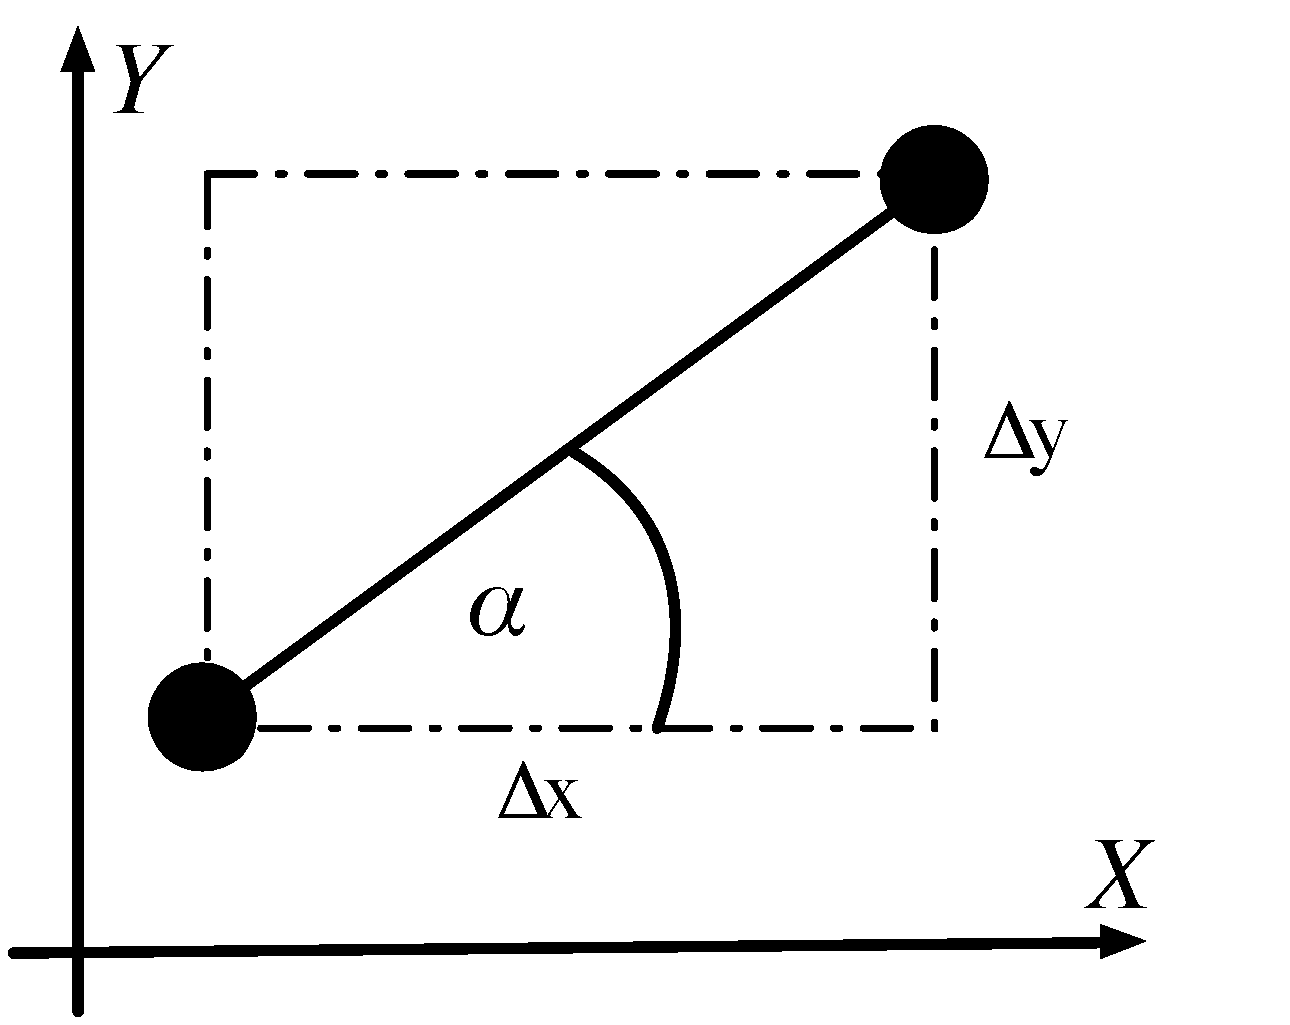
\includegraphics[width=8cm]{rozkladsil.pdf}
\end{center}
\end{frame}

\begin{align*}
    &a_{x}(t) = sin\alpha * a \\
    &a_{y}(t) = cos\alpha * a \\
\end{align*}

Dla przypadku 3D należy rozpatrzyć w analogiczny sposób prostopadłościan (ciała powinny znajdować się w wierzchołkach po przeciwnych ścianach, po przeciwnych rogach).

\section{Model numeryczny}
Interesują nas położenia ciał w kolejnych dyskretnych punktach czasu. Przyjmujemy, że w przeciągu jednostki czasu wielkości prękość, przyśpieszenie są stałe. Aktualizujemy interesujące nas wielkości w kolejności:
\begin{itemize}
    \item 1) aktualizacja prędkości
    \item 2) aktualizacja położenia
    \item 3) aktualizacja przyśpieszenia
\end{itemize}

Co należy podkreślić, wynika z tego, iż do aktualizacji prędkości brana jest poprzednia wartość przyśpieszenia.

Poniżej najistotniejszy fragment kodu w C++ dla CPU. Kod dla przypadku D==2.

\begin{minipage}{\linewidth}
\begin {lstlisting}[language=C++]
/*
    Naming scheme
    @d <- dim index: x == 0, y == 1 or z == 2
    @i <- body index
    @p <- position
    @v <- velocity
    @a <- acceleration

    update variables in order: 1) v, 2) p, 3) a
*/
void NBodiesSystem::step( time_type delta_t ) {
    p_prev = p_curr;
    v_prev = v_curr;

    for (int d = 0; d < D; ++d)
        for (int i = 0; i < N; ++i) {
            v_curr[d][i] = v_prev[d][i]  +  
                a[d][i] * delta_t;
            p_curr[d][i] = p_prev[d][i]  +  
                (v_prev[d][i] + v_curr[d][i]) 
                * 0.5 * delta_t;

            //Bouncing off the wall
            if (p_curr[d][i] > 1 || p_curr[d][i] < -1) 
                v_curr[d][i] = -v_curr[d][i];
        }

    step_a();
} 
\end{lstlisting}
\end{minipage}


\begin{minipage}{\linewidth}
\begin {lstlisting}[language=C++]
void NBodiesSystem::step_a () {
    for (int i = 0; i < N; ++i) {
        for (int j = 0; j < N; ++j) {
            if ( i == j ) continue;

            position_type* r_axis = 
                new position_type[D];
            position_type r_squared = 0;
            for (int d = 0; d < D; ++d) {
                r_axis[d] = 
                    (p_curr[d][i] - p_curr[d][j]);
                r_squared += 
                    r_axis[d] * r_axis[d];
            }

            //To not divide by very small number or zero
            position_type a_scalar = 
                G * m[0][j] / 
                pow(r_squared + efactor, 1.5);

            for (int d = 0; d < D; ++d)
                a[d][i] = 
                    -1 * a_scalar * 
                    (r_axis[d]/r_squared);

            delete [] r_axis;
        }
    }
}
\end{lstlisting}
\end{minipage}

\section{Implementacja GPU}


\section{Wizualizacja: współdziałanie OpenGL i CUDA}


\end{document}